\documentclass{sigchi-ext}
% Please be sure that you have the dependencies (i.e., additional
% LaTeX packages) to compile this example.
\usepackage[T1]{fontenc}
\usepackage{textcomp}
\usepackage[scaled=.92]{helvet} % for proper fonts
\usepackage{graphicx} % for EPS use the graphics package instead
\usepackage{balance}  % for useful for balancing the last columns
\usepackage{booktabs} % for pretty table rules
\usepackage{ccicons}  % for Creative Commons citation icons
\usepackage{ragged2e} % for tighter hyphenation

% Some optional stuff you might like/need.
% \usepackage{marginnote} 
% \usepackage[shortlabels]{enumitem}
% \usepackage{paralist}
% \usepackage[utf8]{inputenc} % for a UTF8 editor only

%% EXAMPLE BEGIN -- HOW TO OVERRIDE THE DEFAULT COPYRIGHT STRIP --
% \copyrightinfo{Permission to make digital or hard copies of all or
% part of this work for personal or classroom use is granted without
% fee provided that copies are not made or distributed for profit or
% commercial advantage and that copies bear this notice and the full
% citation on the first page. Copyrights for components of this work
% owned by others than ACM must be honored. Abstracting with credit is
% permitted. To copy otherwise, or republish, to post on servers or to
% redistribute to lists, requires prior specific permission and/or a
% fee. Request permissions from permissions@acm.org.\\
% {\emph{CHI'14}}, April 26--May 1, 2014, Toronto, Canada. \\
% Copyright \copyright~2014 ACM ISBN/14/04...\$15.00. \\
% DOI string from ACM form confirmation}
%% EXAMPLE END

% Paper metadata (use plain text, for PDF inclusion and later
% re-using, if desired).  Use \emtpyauthor when submitting for review
% so you remain anonymous.
\def\plaintitle{SIGCHI Extended Abstracts Sample File: Note Initial
  Caps} \def\plainauthor{First Author, Second Author, Third Author,
  Fourth Author, Fifth Author, Sixth Author}
\def\emptyauthor{}
\def\plainkeywords{Authors' choice; of terms; separated; by
  semicolons; include commas, within terms only; required.}
\def\plaingeneralterms{Documentation, Standardization}

\title{Prototyping a gesture controlled \underline{H}ead \underline{U}p \underline{D}isplay using a Leap Motion}

\numberofauthors{2}
% Notice how author names are alternately typesetted to appear ordered
% in 2-column format; i.e., the first 4 autors on the first column and
% the other 4 auhors on the second column. Actually, it's up to you to
% strictly adhere to this author notation.
\author{%
  \alignauthor{%
    \textbf{Daniel Brand}\\
    \affaddr{University of Salzburg} \\
    \affaddr{Salzburg, 5020, AUT} \\
    \email{Daniel.Brand@stud.sbg.ac.at} 
}
\alignauthor{%
    \textbf{Kevin B\"uchele}\\
    \affaddr{University of Salzburg}\\
    \affaddr{Salzburg, 5020, AUT}\\
    \email{Kevin.Buechele@stud.sbg.ac.at} 
} \vfil 
}

% Make sure hyperref comes last of your loaded packages, to give it a
% fighting chance of not being over-written, since its job is to
% redefine many LaTeX commands.
\definecolor{linkColor}{RGB}{6,125,233}
\hypersetup{%
  pdftitle={\plaintitle},
%  pdfauthor={\plainauthor},
  pdfauthor={\emptyauthor},
  pdfkeywords={\plainkeywords},
  bookmarksnumbered,
  pdfstartview={FitH},
  colorlinks,
  citecolor=black,
  filecolor=black,
  linkcolor=black,
  urlcolor=linkColor,
  breaklinks=true,
}

% \reversemarginpar%

\begin{document}

\maketitle

% Uncomment to disable hyphenation (not recommended)
% https://twitter.com/anjirokhan/status/546046683331973120
\RaggedRight{} 

% Do not change the page size or page settings.
\begin{abstract}
In todays cars the design of a Head Up Display (HUD) and
the arrangement of its components are rather fixed. This paper provides an approach
how a Leap Motion can be used to achieve a gesture controlled HUD. Furthermore, some aspects that need to be considered
when implementing a modifiable HUD for cars are discussed.
\end{abstract}

\keywords{LeapMotion; HUD; Head Up Display; Automotive; Gesture recognition}

\section{Introduction}
During the last years, the HUD has been established in middle and high class cars.
However, Head Up Displays are often static, in particular, the position of each element in the display
is fixed.

Nowadays, users of any devices appreciate an interface which can be modified.
Since buttons or similar controls may distract the driver from looking at the road,
these types of controlling the interface are bad choices.

After some research, we came to the conclusion that a touchless control
(similar to other approaches to control a infotainment system)
may be a reasonable goal we want to achieve.

A classic device to implement touchless controls is the Leap Motion. We use the Leap Motion
and its gestures which are easy for the user and also easy to be tracked by the device.
In this paper, we will discuss problems and issues we have faced regarding the position of
the Leap Motion, which gestures to use and more important which settings/requirements have to be fixed
in order to get the system working smoothly. By the end, we can select items within a HUD
without any other devices such as a touchpad, knobs etc.

\section{The system's environment}
The Leap Motion is a classic sensor device to track the hands of a user and therefore the gestures of the users hands.
The detection of the hand works with an infrared camera which has the advantage that noise in the information, generated by the environment light, 
is reduced. The sensor recognizes each finger including
bones and joints. So far, our system has been configured to work with a right hand only.

\FloatBarrier

\begin{figure}
\centering
  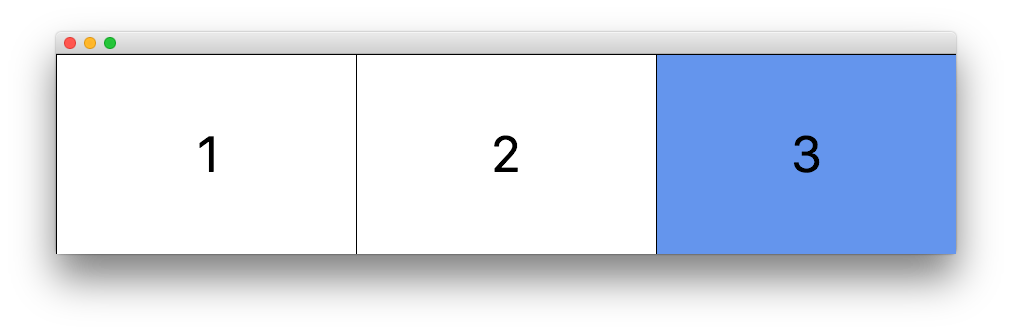
\includegraphics[width=0.9\columnwidth]{figures/hudelements.jpg}
  \caption{Simulated HUD with 3 elements. User is pointing at element 3.}~\label{fig:figure1}
\end{figure}

Our HUD will be simulated with the the JavaFX framework. In order to test which settings fit the most for this use,
we are able to dynamically display 3 or 4 elements in our HUD, simply represented with numbers between 1 and 3 (respectively 4).
Certain gestures above the Leap Motion will cause an interaction with the JavaFX window.
The Leap Motion is set up to track 2 major gestures: pointing at a certain field (see figure)
and selecting it by moving the pointing finger slightly in direction to the HUD. The current marked element will get a blue background, while the selected element will be shown with a green background. In the case of our prototype,
the Leap Motion framework and the JavaFX framework are running on the same computer.

The angles between the index finger, in our test setup the vertical y axis, and the HUD, horizontal x axis,  has to be adapted accordingly. This is because we are using the
interface with the right hand, more specifically the right index finger, only. Obviously, the anatomy of our hand
allows a slightly bigger movement range of the right index finger to the left instead of the right. This needed some testing, and we came to
the conclusion that the angles have to be adapted within the program in order to achieve a satisfying control of the HUD. We use a more accurate granularity of the interval angles on the 
right side.

\section{Test setup}
Our test setup was built up in the driving simulator of the HCI-Center in Salzburg. A small netbook running eclipse executes the program and simulates our HUD. The Leap Motion which is plugged into this netbook is placed right behind the steering wheel. It has to be mentioned that we did not use a standard sized steering wheel. Instead, we used a more flattened steering wheel which is quite similar to steering wheels of modern (self driving) cars such as Tesla.

\FloatBarrier

\begin{figure}
\centering
  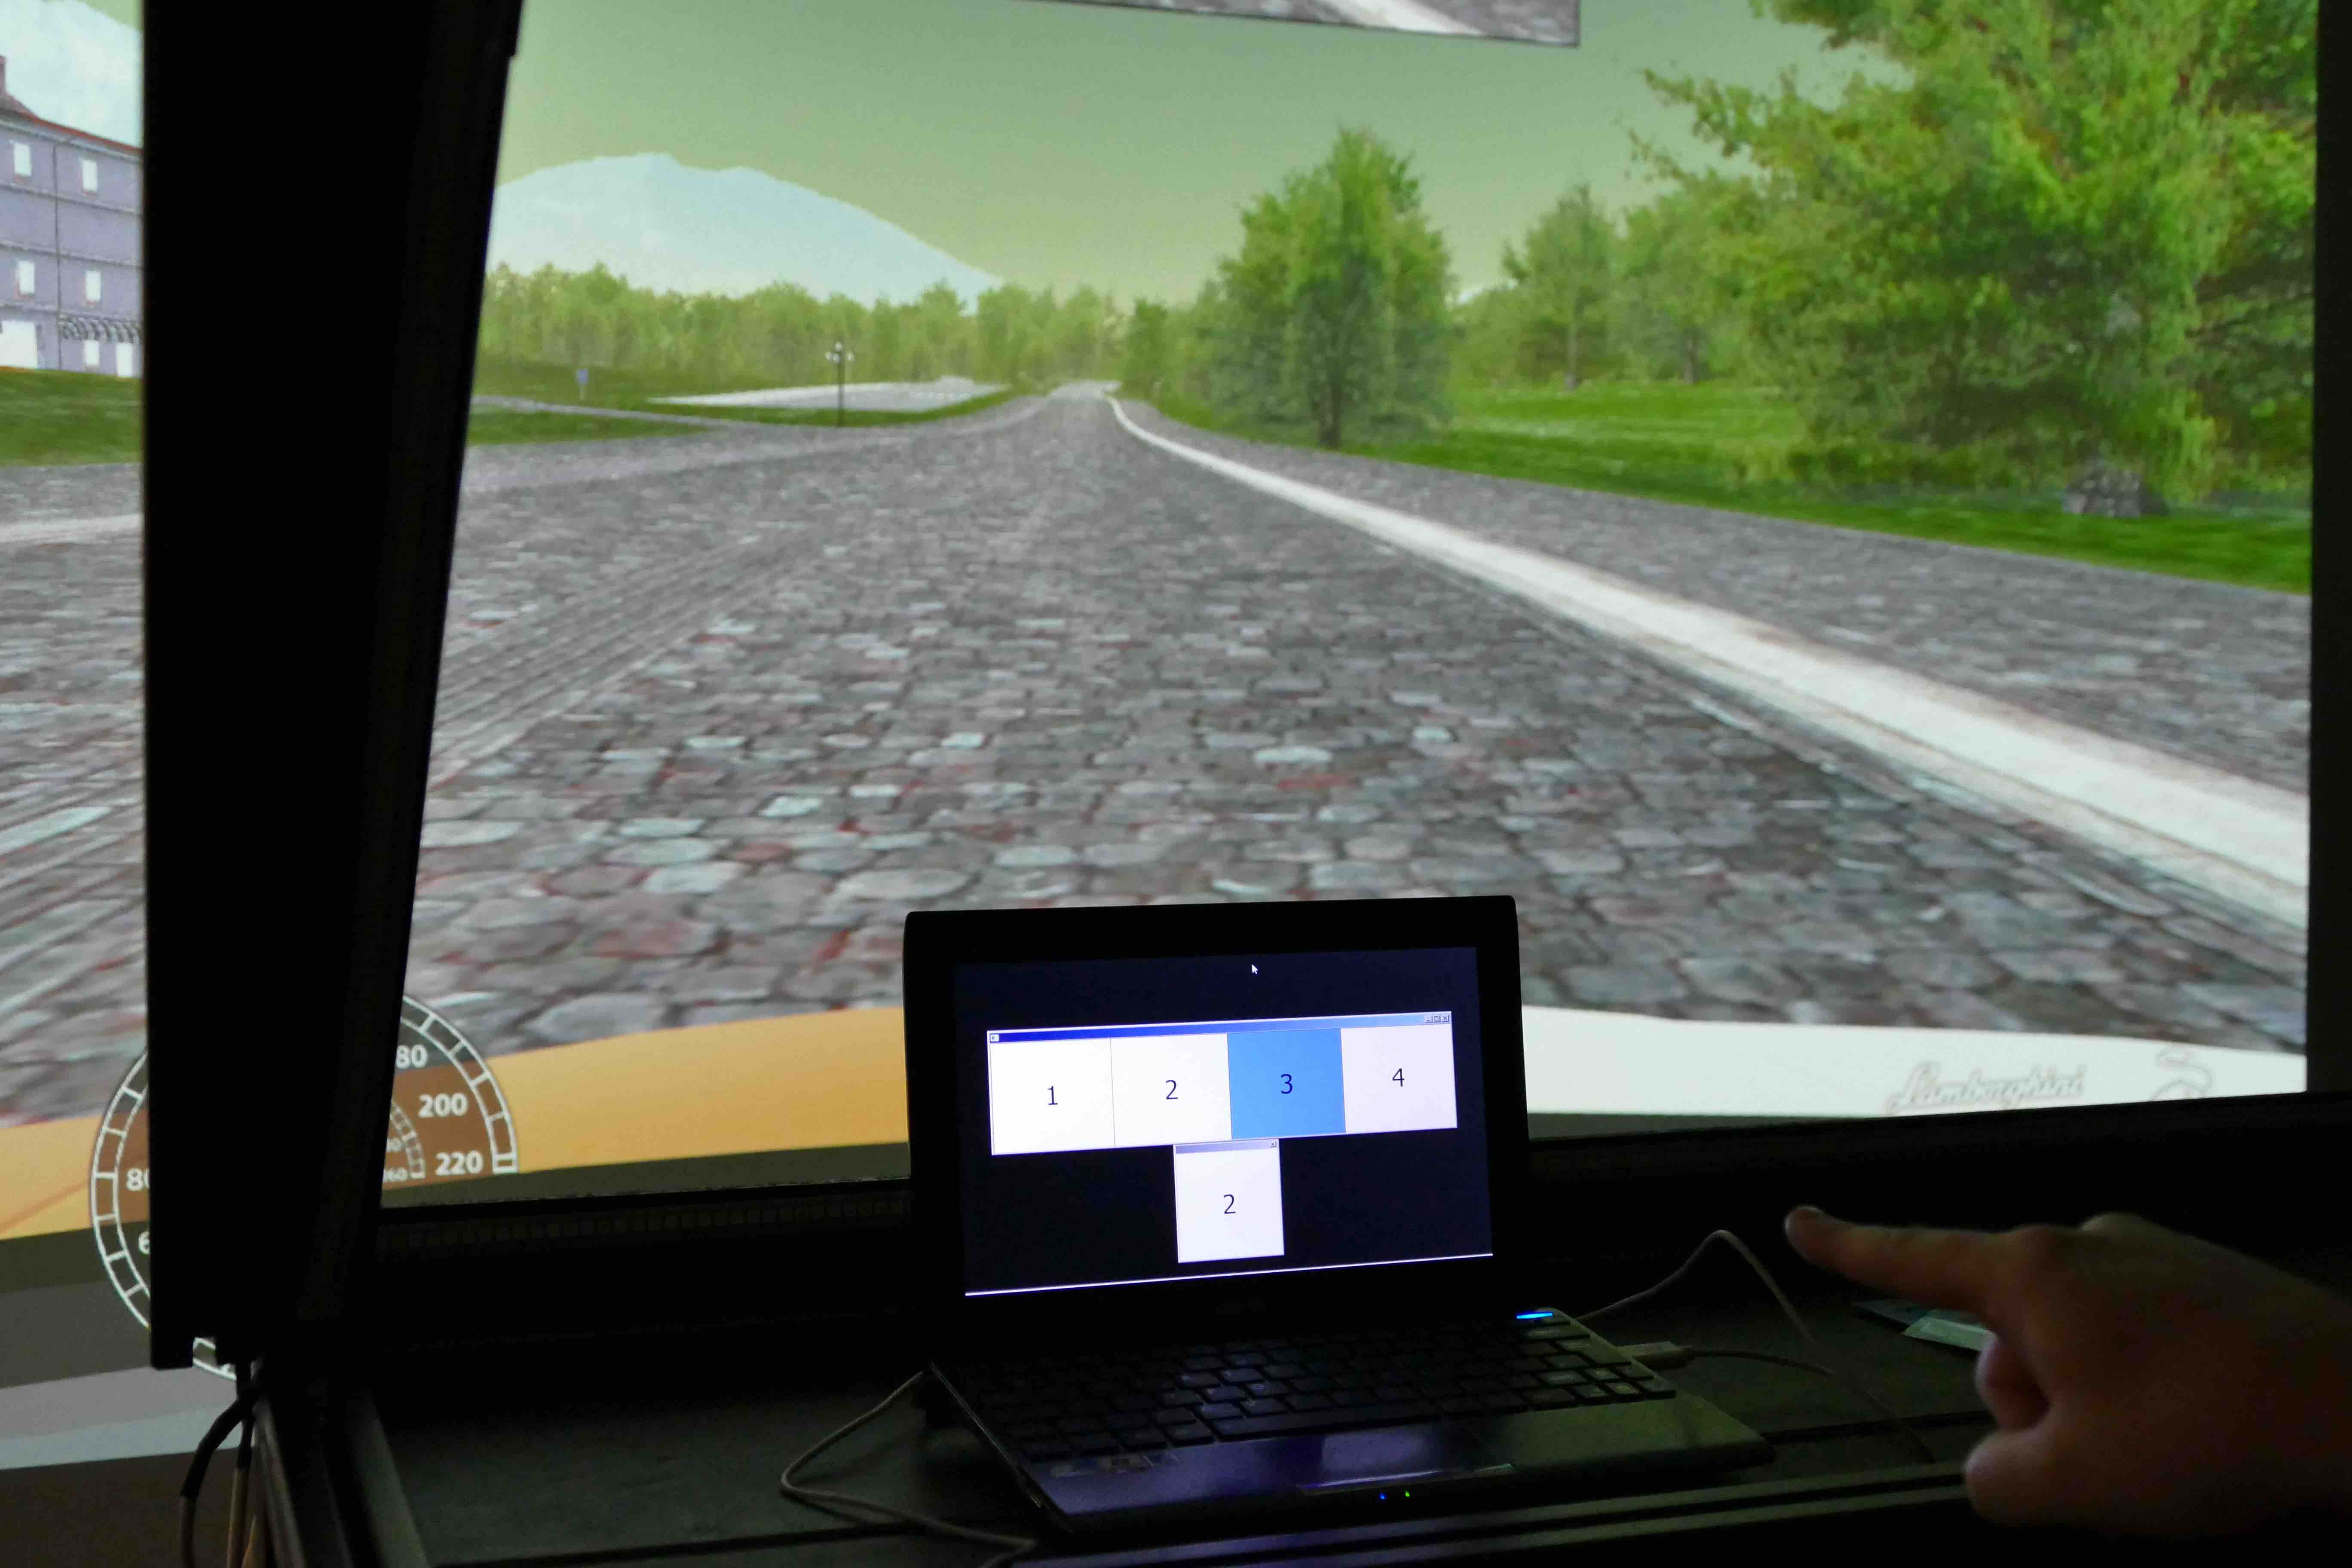
\includegraphics[width=0.9\columnwidth]{figures/testsetup.jpg}
  \caption{Test setup during the case studies with the driving simulator. }~\label{fig:figure1}
\end{figure}

Each test person needs to complete two test sessions. The difference between this sessions is the amount of elements in our HUD. After some pre-tests, we now only include test sessions with three and four elements. Using five elements did not lead to pleasant results since selecting one out of five elements was way too difficult.

Each session consists of 15 steps. Steps are the same for every test. In each step, the program shows a random number in a small window below the HUD. The user now has to try and select the shown element by moving the index finger accordingly (left or right). If the desired element is marked, the user can then select it by moving the pointing finger slightly forward (screen tap gesture). After successfully (or not) selecting an element, the test sequence is continued after a small delay of 3500 ms with the next element.

Between each step, the user has to put his hand back to the steering wheel again. This makes sure that his hand does not keep on pointing onto the selected element which would make the next selection easier if the same element has to be selected. Furthermore, we think it is more realistic when the user's hand has to be moved from the steering wheel to the HUD.

Throughout the whole test, the user also has to keep driving with the driving simulator. We want our test setup to be as realistic as possible. 

The result of each step is recorded and (after completing the sequence) summarized in a log file. The logfile provides detailed test results in order to validate our prototype. The first few lines give a summary about basic settings and results such as implemented angles, test sequence, touched elements in the test sequence and the duration of the whole test. The second bigger a part of the log file gives an exact result about which angle was hit after each step (with respect of the angle window of the element). Also an error rate over all selected (or missed) elements is written into the logfile.

\section{Test results}
The test session was performed by ten participants.  Each participant could practice driving the simulator while selecting some elements in our HUD. It was obvious that each test person got familiar with the control faster than expected. This showed that our chosen gestures seem to be very intuitive and useful for the majority of people.

The test session with 3 selectable elements gives us better results (see table 1). After evaluating all test results, we saw that the error rate was lower in this case. The reason is simple: the HUD is configured to track angles between 0 and 180 degrees independent from the amount of elements to be selected. This means that this range only needs to be split into 3 intervals (instead of 4). Another thing that has to be considered is the time that was needed to perform the test. Again, the test session with 3 elements seems to be more successful. The average time that was needed is significantly lower compared to the test with 4 elements. 

\begin{table}
\begin{tabular}{|l|l|l|}
\hline
  & \textbf{HUD with 3 elements} & \textbf{HUD with 4 elements} \\
\hline
\textbf{Avg. time} & \textit{109 seconds} & \textit{199 seconds} \\
\hline
\textbf{Avg. error rate} & \textit{18,1 \%} & \textit{24,8 \%} \\
\hline
\end{tabular}
\caption{Test results with 3 and 4 elements}
\end{table}

Some other interesting results are summarized in table 2 and table 3. It is obvious that the average hit points on 4 elements are rather close to the interval borders compared to the results with 3 elements. Combined with the error rates in table 1, we can (again) conclude that selecting one of 4 elements is more difficult than selecting one of 3. Again, this was the reason why we excluded the test session with 5 elements as we did not see any chance for a satisfying success in this case.

After talking to the participants and evaluating the short questionnaire we created for this purpose, we can summarize that our system seems to be rather intuitive to use and has potential to be used in the future. However, it was also mentioned that the system may distract the driver too much. Therefore, further and more detailed tests might have to be made to fix this thesis. Maybe changes to the system would have to be considered as well, but this is not part of our work.

\begin{table}
\begin{tabular}{|l|l|l|l|}
\hline
  & \textbf{Element 1} & \textbf{Element 2} & \textbf{Element 3} \\
\hline
\textbf{Angle interval} & \textit{180$^\circ$ - 100$^\circ$} & \textit{100$^\circ$ - 80$^\circ$} & \textit{80$^\circ$ - 0$^\circ$} \\
\hline
\textbf{Avg. hit point} & \textit{110,43$^\circ$} & \textit{92,54$^\circ$} & \textit{75,63$^\circ$} \\
\hline
\end{tabular}
\caption{Hit points when using 3 elements}
\end{table}

\begin{table}
\begin{tabular}{|l|l|l|l|l|}
\hline
  & \textbf{Element 1} & \textbf{Element 2} & \textbf{Element 3} & \textbf{Element 4} \\
\hline
\textbf{Angle interval} & \textit{180$^\circ$ - 100$^\circ$} & \textit{100$^\circ$ - 95$^\circ$} & \textit{95$^\circ$ - 85$^\circ$} & \textit{85$^\circ$ - 0$^\circ$} \\
\hline
\textbf{Avg. hit point} & \textit{108,97$^\circ$} & \textit{97,29$^\circ$} & \textit{88,91$^\circ$} & \textit{78,67$^\circ$} \\
\hline
\end{tabular}
\caption{Hit points when using 4 elements}
\end{table}

\section{Conclusion}
Our approach provides an interesting and new way of interaction between the car and its driver. 

The main goal of our prototype was to figure out which system settings are the best for a comfortable control of a HUD. In our opinion, we came to a satisfying result regarding this goal. When it comes to the angle intervals, one has to mention that they might differ from car to car as they depend on the location of the Leap Motion. Regarding gestures, we tried to find a set of those that are recognized by the Leap Motion in a satisfying rate.

However, there is still some room for improvements such as different gestures. Furthermore, more functionalities can be added in case of future studies on this topic.

\bibliographystyle{SIGCHI-Reference-Format}
\bibliography{sample}

\end{document}

%%% Local Variables:
%%% mode: latex
%%% TeX-master: t
%%% End:
